% -*-coding: utf-8;-*-
%%%%%%%%%%%%%%%%%%%%%%%%%%%%%%%%%%%%%%%%%%%%%%%%%%%%%%%%%%%%%%%%%%%%%%%%%%%%%%
% Программный комплекс для обучения методам нейросетевого управления в
% учебном процессе

% План:
% 1. Мотивация
%  1.1. Важность практических занятий в освоении НС
%  1.2. Почему новый пакет?
%  1.3. Состав лабораторных работ
%  1.4. Дидактические аспекты
% 2. Описание пакета
%  2.1. Перечень функций (смысловых, интерактивных)
%  2.2. Архитектура пакета
%  2.3. Выбор программной платформы
%  2.4. Описание объектной библиотеки и программ
% 3. Описание лабораторных работ
%  3.1. Синтез нейросетевого регулятора
%  3.2. Сравнение НС-Р, винервского оптимального и ПИД регулятора
%  3.3. Нейросетевое управление нестационарным объектом

\section{Цель работы}

Применение нейронных сетей в системах управления является достаточно
новым направлением.  Исследования в этой области идут широким фронтом,
однако методологические аспекты пока недостаточно проработаны.  В
частности, это сказывается на том, что отсутствуют общеизвестные
программные пакеты, позволяющие без программирования изучать
нейросетевые методы автоматического управления.  Нет подходящих для
этого и web-ресурсов.

В то же время, теоретический базис по нейронным сетям на настоящий
момент не дает обоснованных конструктивных путей решения прикладных
задач.  Это делает применение нейронных сетей во многом эвристическим
процессом.  В таких условиях ВУЗовский учебный курс по нейронным сетях
обязательно должен включать практические занятия, позволяющие
студентам разобраться в недостаточно формализованном предмете и
получить необходимый опыт.

Представляется актуальным разработать интерактивный программный
комплекс для настройки и моделирования традиционных и нейросетевых
систем управления с обратной связью.  Подобный комплекс был бы полезен
как в рамках учебного процесса к курсе нейронных сетей и курсе систем
автоматического управления на инженерных специальностях ВУЗов, так и в
инженерной практике при проектировании несложных систем управления.

\section{Основные решаемые задачи}

В соответствии со своим назначением программный пакет должен решать
задачи моделирования САУ, моделирования и обучения нейронных сетей.
Типовой сеанс работы с пакетом подразумевает интерактивное
взаимодействие пользователя с программами.  Поскольку пакет
разрабатывается для применения в учебном процессе, весьма желательно,
чтобы он был:
\begin{itemize}
\item простым в изучении и использовании;
\item адаптированным к специфике учебного процесса;
\item открытым к модификации;
\item основанным на открытых технологиях.
\end{itemize}

При моделировании систем автоматического управления необходимо
предусмотреть возможность гибкой настройки контура и условий его
работы.  В частности, должны настраиваться:
\begin{itemize}
\item уставка (стохастическая, детерминированная);
\item помеха (стохастическая, детерминированная);
\item регулятор (линейный, нейросетевой);
\item объект управления (линейный, нелинейный, нестационарный).
\end{itemize}

В то же время, учитывая учебную направленность пакета, представляется
достаточным ограничиться одномерными системами управления когда объект
является одноканальным по входу и выходу.  Это существенно упрощает
интерактивную часть пакета и практику его использования.

Для моделирования и обучения нейронных сетей должны присутствовать
следующие возможности:
\begin{itemize}
\item создание нейронной сети с произвольной архитектурой в классе
  многослойных персептронов;
\item обучение нейронной сети на обучающей выборке с контролем
  процесса по тестовой выборке;
\item предсказание поведения объекта управления с помощью нейронной
  сети в контуре управления в процессе моделирования;
\item обучение нейронной сети регулятора в контуре управления в
  процессе его моделирования.
\end{itemize}

Специфика применения нейронных сетей в системах автоматического
управления заключается в преимущественном использовании сетей класса
многослойный персептрон с обучением методом обратного распространения
или более эффективными его вариантами.  По этой причине
нецелесообразно реализовывать поддержку сетей иных архитектур
(Кохонена, Хопфилда и пр.).  Применяемые в САУ нейронные сети,
основанные на радиально-базисных функциях (RBF), доказанно являются
эквивалентными многослойному персептрону, поэтому их реализация тоже
является избыточной и ради простоты программного комплекса от неё
целесообразно отказаться.

\section{Интеграция в учебный процесс и дидактические аспекты}

\subsection{Мотивация}

%  1.1. Важность практических занятий в освоении НС

Искусственные нейронные сети представляют собой относительно новый
мощный и многогранный инструмент для решения разнообразных инженерных
и научно-исследовательских задач.  Способ применения нейронных сетей
достаточно специфичен, так как он основан не на аналитическом
формализме, являющемся результатом работы человеческого интеллекта, а
на машинном обучении --- неявном извлечении взаимосвязей из
представленных данных.  Эта особенность отличает нейросетевые методы
от традиционных, в том числе и в задачах автоматического управления.

Аналитические методы давно и прочно укоренились в учебных курсах на
инженерных специальностях.  Для освоения аппарата этих методов
студентам предлагается большое количество разнообразных упражнений,
суть которых сводится к аналитическому решению задачи, то есть, к
выводу формальным способом решения в общем виде.  Только в том случае,
если математический аппарат не позволяет получить точное решение в
аналитической форме, используются приближенные способы решения, в том
числе, с помощью численных методов.  Однако в любом случае вид
решения, а значит и его свойства, определяются человеком.

Нейросетевые методы подразумевают участие человека только в
обеспечении процесса обучения, а собственно решение формируется
нейросетью само.  Его вид и свойства изначально неизвестны.  Более
того, после успешного завершения обучения нейронной сетью, отличной от
тривиальной, человеку практически невозможно понять, какие решения
приняла сеть и как это повлияло на достижение поставленной цели.
Извлечение знаний из обученной нейронной сети представляет собой
отдельную проблему.

Причину этого следует искать в том, что существующая на настоящий
момент теория искусственных нейронных сетей неполна.  В частности, не
существует математически доказанных конструктивных методов,
обеспечивающих решение базовой задачи: интерполяции произвольной
функции нейросетью.  Вопросы информационной ёмкости нейронной сети
решены только для небольшого класса сетей с линейными нейронами,
бесперспективность которого была показана ещё в 1960-х годах Мински
(???).  Архитектура и принципы функционирования нейронных сетей разных
типов чрезвычайно разнообразны, а математический аппарат, используемый
в нейросетевых методах решения прикладных задач, позаимствован из
разных областей прикладной математики.

Возможность применения нейронных сетей основывается только на теореме
(???) о существовании решения интерполяции произвольной функции
многослойным нелинейным персептроном.  В отсутствии теоретически
обоснованного конструктивного метода настройки нейронной сети широкое
распространение получили различные численные методы, близкие к
нелинейной оптимизации, а также разнообразные эвристические подходы.

Изложенные особенности свидетельствуют об особой важности практических
работ в учебном курсе по нейросетевым методам.  Только они дают
возможность студентам увидеть, как происходит процесс обучения и как
функционирует обученная нейронная сеть в рамках решения конкретной
прикладной задачи.  Это невозможно до конца формализовать на лекциях и
изложить в учебных пособиях.  Фактически, совокупность архитектуры НС,
метода обучения с его параметрами, а также обучающих данных дает
уникальное решение, выражающееся в наборе весовых коэффициентов НС.

%  1.2. Почему новый пакет?

Обычно для практических работ по курсу искусственных нейронных сетей
используется тот или иной универсальный (Statistica, MatLab, Octave)
или специализированный нейросетевой (Stuttgart Neural Network
Simulator, Neural Lab, Trajan) программный пакет.  Для большинства
типовых задач, решаемых с помощью НС (распознавание образов,
ассоциативная память, кластеризация, предсказание и т.п.),
возможностей перечисленных пакетов вполне достаточно.  К ним
относятся:

\begin{itemize}
\item Задание архитектуры нейросети и метода её обучения
\item Задание обучающего множества
\item Задание параметров обучения
\item Обучение нейронной сети
\item Анализ качества работы обученной нейронной сети
\end{itemize}

Однако применение НС в задачах управления требует дополнительно
наличия многих функций, отсутствующих в пакетах нейросетевого
моделирования:

\begin{itemize}
\item Задание вида и параметров регулятора и объекта управления
\item Задание входных сигналов - уставки и помехи
\item Съем данных из различных точек контура управления для
  визуализации и обучения НС
\item Моделирование САУ
\item Сравнение и анализ качества работы САУ с различными
  компонентами, в том числе, с нейросетевыми
\end{itemize}

В универсальных пакетах (класса MatLab) реализация перечисленных
функций требует достаточно серьезного программирования как
вычислительных, так и интерактивных и графических функций.  В то же
время, получающаяся программа обладала бы ограниченным
быстродействием, так как должна быть написана на интерпретируемом
языке программирования.  Вопросы быстродействия в классе задач
автоматического управления достаточно важны, так как моделирование и
обучение нейронных сетей производится на длинных временных рядах
(порядка $10^4 ... 10^6$ отсчетов).

Ещё одним классом программ, разрабатываемым в учебных целях, являются
демонстрационные программы чаще всего размещаемые с Интернете и
доступные для online-использования (??? привести перечень ссылок).
Такие программы обычно демонстрируют какой-то конкретный алгоритм
управления на конкретном объекте, например, управление обратным
маятником, поэтому рядом с online-интерфейсом программы расположено
описание алгоритма управления, системы или ссылки на такую информацию.
Для проведения моделирования пользователю достаточно запустить систему
моделирования.  Иногда имеется возможность задать некоторые параметры
системы и возмущающее воздействие.  Для наглядной демонстрации работы
САУ используется динамическая графика и, в целом, оформление сделано
весьма эффектно.  К достоинствам online-программ относится то, что их
не надо устанавливать на компьютер, они не потребляют компьютерных
ресурсов пользователя (за исключением web-браузера, используемого для
доступа на web-страницу программы) и доступны везде и всегда где есть
доступ в Интернет.

В то же время, у подобных программ, часто выглядящих как рекламный
ролик алгоритма управления, есть свои недостатки:
\begin{itemize}

\item узкая специализация на одной прикладной задаче, причем часто
  даже с фиксированными параметрами;

\item презентационная направленность, скрывающая от пользователя
  ``скучные'' элементы алгоритма и демонстрирующие только результат;

\item обычно отсутствует возможность сравнения с иными алгоритмами
  управления.

\end{itemize}

Таким образом, демонстрационные online-программы могут быть
использованы в учебном процессе очень ограниченно --- для иллюстрации
работы конкретных управляющих алгоритмов в конкретных задачах.  Для
практических занятий, подразумевающих деятельное участие студентов,
они совершенно непригодны.

Представляется актуальным разработать интерактивный пакет программ,
позволяющий решать задачи нейросетевого управления и сопоставлять
нейросетевые подходы с традиционными.  На базе такого пакета можно
создать курс практических занятий для студентов инженерных
специальностей, изучающих нейросетевые методы вообще и применение
нейронных сетей в системах автоматического управления в частности.

Расширение лабораторной базы учебного процесса позволит укрепить
знания, получаемые студентами на лекциях, практическим опытом решения
учебных задач.  

При определенной гибкости настроек подобный программный комплекс был
бы полезен и для исследовательских проектов, позволяя быстро проводить
моделирование проектируемой САУ и оценивать возможности использования
в ней нейросетевого управления.

%  1.3. Состав лабораторных работ

Разрабатываемый курс лабораторных работ предназначен для расширения
существующего курса, посвященного применению искусственных нейронных
сетей.  В рамках имеющихся ограничений по времени на нейросетевые
системы управления выделено три практических занятия длительностью
3--4 часа каждое.  Представляется оптимальным скомпоновать учебный
материал в занятия по следующим темам:

\begin{itemize}
\item Синтез нейросетевого регулятора.
\item Сравнительный анализ нейросетевого, винеровского и ПИД регуляторов.
\item Нейросетевое управление нестационарным объектом.
\end{itemize}

Первая лабораторная работа посвящается методике замены регулятора в
существующей системе управления на нейросетевой.  Для этого необходимо
провести моделирование и собрать данные для начального обучения
нейросетевого регулятора и модели объекта.  После этого требуется
настроить нейронные сети регулятора и модели объекта.  Предварительно
настроенный регулятор включается в САУ на место исходного и с помощью
модели объекта в процессе работы подстраивается для минимизации ошибки
управления.

В рамках второй работы требуется сравнить настроенный нейросетевой
регулятор с винеровским оптимальным и ПИД-регулятором в различных
условиях, как эталонных (используемых при настройке), так и
отличающихся от них.  В частности, следует провести моделирование с
разными типами сигналов уставки и интенсивностью помехи,
экспериментально исследовать зависимость качества управления от
частоты, определить, насколько чувствителен регулятор к точности
задания параметров объекта управления.

Третья лабораторная работа посвящена задаче нейросетевого управления
нестационарным объектом.  Она включает настройку системы обнаружения
разладки, сбор данных и подстройку с их помощью модели объекта
управления, а также подстройку нейросетевого регулятора в контуре.

%  1.4. Дидактические аспекты

Успешное выполнение практической работы требует от студента следующих
видов деятельности:

\begin{itemize}

\item изучение теоретических основ нейронных сетей;

\item освоение программного комплекса;

\item подготовку отчета.

\end{itemize}

Материал, вошедший в лабораторные работы, подразумевает, что помимо
теоретических знаний лекционной части курса студент обладает знаниями
по математической статистике, теории функций комплексного переменного
и линейной теории автоматического управления (для детерминированных и
стохастических сигналов).

В результате выполнения практических работ студент должен изучить:
\begin{itemize}

\item Архитектуру нейронных сетей прямого распространения.

\item Способы реализации нейронными сетями динамических свойств
  элементов системы автоматического управления ($\{{e_k,r_k}\}$,
  $\{e_k,e_{k-1},...\}$, $\{u_k,u_{k-1},...y_k,y_{k-1},...\}$).

\item Влияние выбранного критерия качества управления, используемого
  при настройке регулятора, на функционирование САУ в условиях,
  приближенных к реальным (помеха, неточная параметризация сигналов и
  объекта управления, нестационарность).

\item Метод обратного распространения ошибки и его применение при
  синтезе элементов нейросетевой системы управления (начальная
  настройка и подстройка в контуре нейросетевого регулятора, настройка
  нейросетевой модели объекта управления).

\item Роль нейросетевой модели объекта при синтезе нейросетевого
  регулятора и при обнаружении разладки.

\item Влияние обучающих и контрольных данных на свойства обученной
  нейронной сети (область определения и область значений нейросети).

\item Основные свойства нейросетевых регуляторов и их отличия от
  линейных регуляторов (частотная характеристика, зависимость от
  уровня сигналов, устойчивость, адаптированность к нелинейным
  объектам и пр.).

\item Методы нейросетевого управления нестационарным объектом и их
  особенности (быстродействие, ресурсоемкость, устойчивость).

\end{itemize}

Совершенствование лабораторной базы.  Предлагается создать лабораторные работы.

Программный комплекс.
Задачи, возложенные на этот комплекс.

\subsection{Структура комплекса}

\begin{figure}
\centerline{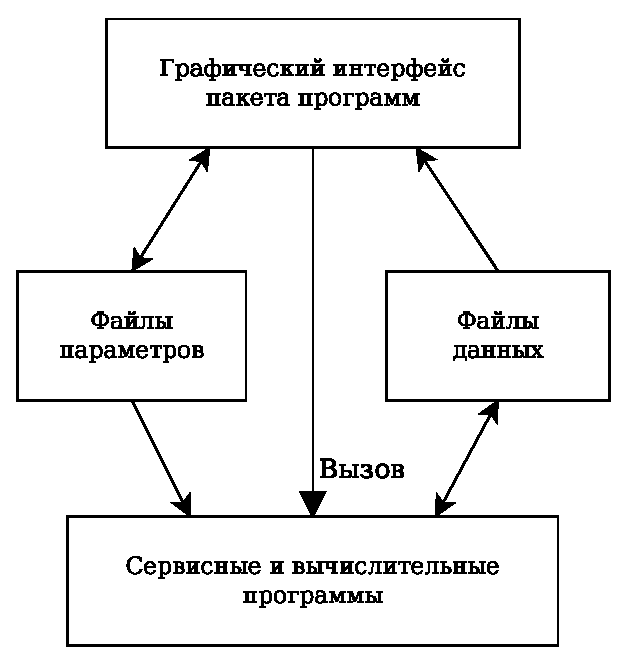
\includegraphics{princ_struct.eps}}
\caption{Схема взаимодействия частей программного комплекса}
\label{fig:prog_interaction_struct}
\end{figure}

\subsection{Функциональная декомпозиция}

Функционально пакет должен обеспечивать решение следующих основных
задач:
\begin{enumerate}
\item Моделирование САУ с возможностью гибкого задания вида уставки,
  помехи, регулятора и объекта управления.  Необходимо предусмотреть
  возможность моделирования нестационарных и нелинейных объектов
  управления, а также использование нейронных сетей.
\item Создание и обучение нейронных сетей как в контуре, так и вне
  контура САУ.
\end{enumerate}

\begin{itemize}
\item Задание архитектуры нейросети и метода её обучения
\item Задание обучающего множества
\item Задание параметров обучения
\item Обучение нейронной сети
\item Анализ качества работы обученной нейронной сети
\end{itemize}

Однако применение НС в задачах управления требует дополнительно
наличия многих функций, отсутствующих в пакетах нейросетевого
моделирования:

\begin{itemize}
\item Задание вида и параметров регулятора и объекта управления
\item Задание входных сигналов - уставки и помехи
\item Съем данных из различных точек контура управления для
  визуализации и обучения НС
\item Моделирование САУ
\item Сравнение и анализ качества работы САУ с различными
  компонентами, в том числе, с нейросетевыми
\end{itemize}


\subsection{Принципы взаимодействия}


\section{Описание лабораторных работ}

\subsection{Синтез нейросетевого регулятора}

\subsubsection{Цель работы}

Лабораторная работа посвящена задаче синтеза нейросетевого
оптимального регулятора.  В ней изучаются принципы применения
нейронных сетей в качестве регулятора и модели объекта управления.
Исследуется влияние архитектуры нейронной сети на скорость и качество
обучения.  Полученный нейросетевой оптимальный регулятор используется
в последующих лабораторных работах.

\subsubsection{Постановка задачи}

Имеется система управления с обратной связью.  У объекта управления
один управляющий вход и один наблюдаемый выход.  Известно, что в
канале наблюдения имеется случайная помеха.  Дана стохастическая
модель сигнала уставки.  Необходимо заменить регулятор на нейросетевой
с минимизацией квадрата ошибки управления.

Для простоты понимания задачи и в целях последующего сравнения с
линейными регуляторами в качестве объекта управления и регулятора
берутся линейные звенья, хотя методика синтеза никак не ограничивает в
выборе класса управляемого объекта и заменяемого регулятора.

В процессе выполнения промежуточных этапов синтеза исследуется влияние
архитектуры нейронной сети (количество слоев, распределение нейронов в
них) на скорость обучения и достигаемое качество.

\subsubsection{Варианты}

Различные варианты данной работы можно обеспечить, задавая разные
параметры объекта управления, уставки и помехи.

\subsubsection{План работы}

Работа состоит из последовательного выполнения следуюих подзадач:
\begin{enumerate}
\item Моделирование САУ с линейным регулятором в контуре с целью сбора
  данных для обучения нейронных сетей.
\item Задание архитектуры нейросетевой модели объекта управления.
\item Обучение нейросетевой модели предсказанию наблюдаемого выхода
  объекта управления.
\item Повторить два предыдущих пункта для разных архитектур нейронных
  сетей.  Выбрать наилучший по минимуму ошибки предсказания на
  тестовой выборке.
\item Задание архитектуры нейросетевого регулятора.
\item Обучение нейросетевого регулятора функционированию подобно
  исходному вне контура управления.
\item Повторить два предыдущих пункта для разных архитектур нейронных
  сетей.  Выбрать наилучший по минимуму ошибки имитации на тестовой
  выборке.
\item Замена исходного регулятора нейросетевым в контуре управления и
  включение контура его адаптации с помощью нейросетевой модели.
\item Моделирование САУ с обученным нейросетевым регулятором в контуре
  с целью сравнения его с исходным.
\end{enumerate}

\subsubsection{Пример отчета}


\subsection{Сравнение нейросетевого, винеровского оптимального и ПИД регулятора}

\subsubsection{Цель работы}

Работа посвящена исследованию свойств нейросетевого регулятора в
сравнении с линейными регуляторами: универсальным и широко
используемым в промышленной автоматике ПИД регулятором и винеровским
--- оптимальным в случае линейной САУ.  Сравнение регуляторов
проводится в различных условиях на основе интегрального
(среднеквадратичная ошибка) и экстремального (максимальная ошибка)
критериев.

\subsubsection{Постановка задачи}

Имеется система управления с обратной связью и линейным объектом
управления.  Стохастические параметры уставки и помехи заданы.  Для
системы синтезированы ПИД регулятор, винеровский оптимальный регулятор
\footnote{Линейный объект должен иметь вид, допускающий существование
  физически реализуемого винеровского оптимального регулятора} и
нейросетевой квазиоптимальный регулятор, например, полученный во время
первой лабораторной работы.

Сравнение регуляторов следует проводить исходя из достигнутого ими
качества управления на достаточно длинном временном интервале.
Критериями качества управления являются максимальное по модулю
перерегулирование и среднеквадратичная ошибка.

Требуется экспериментально исследовать поведение трех видов
регуляторов в номинальных условиях, на разных видах сигнала уставки
(ступенчатом, гармоническом, стохастическом), а также в условиях,
отличных от номинальных: иные параметры объекта управления, уставки и
помехи (отсутствие, номинальный уровень, повышенный уровень помехи,
``цветная'' помеха).  Экспериментально определить зависимость качества
управления от частоты, подавая на вход системы гармоническую уставку.

\subsubsection{Варианты}

Данная работа может выполняться по вариантам заданных САУ (параметры
ОУ, уставки и помехи), а также по набору экспериментов, которые
следует провести.

\subsubsection{План работы}

Каждый пункт плана работы подразумевает независимый от других пунктов
сеанс моделирования для каждого из трех видов регуляторов.  Перед этим
необходимо подготовить сигналы уставки и помехи, а также установить
параметры объекта управления сообразно заданию.

\begin{enumerate}
\item Номинальная стохастическая уставка и помеха, номинальный объект
  управления.
\item Уставка --- меандр с длительностью ступеней, достаточной для
  завершения переходного процесса.  Помеха --- отсутствует.  Объект
  управления --- номинальный.
\item Уставка --- синусоида.  Помеха --- отсутствует.  Объект
  управления --- номинальный.  Повторить для нескольких различных
  частот уставки , включая частоту Найквиста.
\item Стохастическая уставка, отличная от номинальной с дисперсией,
  примерно совпадающей с номинальной.  Номинальная помеха.  Объект
  управления --- номинальный.
\item Стохастическая уставка, отличная от номинальной с дисперсией, в
  два раза превышающая номинальную.  Номинальная помеха.  Объект
  управления --- номинальный.
\item Номинальная стохастическая уставка.  Помеха --- белый шум с
  интенсивностью в два раза больше, чем номинальная.  Объект
  управления --- номинальный.
\item Номинальная стохастическая уставка.  Помеха --- ``цветной'' шум.
  Объект управления --- номинальный.
\item Номинальная стохастическая уставка и помеха.  Параметры объекта
  управления отличаются от номинальных.
\item Номинальная стохастическая уставка и помеха.  Вид объекта
  управления отличается от номинального.
\end{enumerate}

\subsubsection{Пример отчета}


\subsection{Нейросетевое управление нестационарным объектом}

\subsubsection{Цель работы}

Практическая работа нацелена на построение нейросетевой системы
управления нестационарным объектом.  Рассматриваются вопросы
обнаружения разладки с помощью нейросетевой модели объекта и алгоритма
куммулятивных сумм (АКС), сбора обучающих данных и адаптации
регулятора в контуре.

\subsubsection{Постановка задачи}

Рассматривается задача адаптации нейросетевого регулятора при
обнаружении изменений в поведении объекта управления.  Считаем, что
изменения происходят достаточно редко и ступенчато.  Уставка и помеха
являются стохастическими и не меняющими своих свойств.

Кроме нейросетевого регулятора имеется также нейросетевая модель
объекта управления, работающая параллельно с объектом и выдающая
предсказание его выхода.  Разность предсказания и выхода является
ошибкой идентификации.  При обнаруженном росте дисперсии этой ошибки
считается установленным факт разладки, то есть, изменения объекта
управления.  Нейросетевой регулятор и модель объекта получены в ходе
первой лабораторной работы.

Для обнаружения разладки по дисперсии ошибки идентификации применяется
алгоритм куммулятивных сумм, настраиваемый с целью обеспечить
компромисс между минимизацией среднего времени запаздывания при
обнаружении разладки и максимизацией среднего времени между ложными
тревогами.  Основными управляемыми параметрами АКС являются порог
(решающая граница) и номинальная разладка.

После обнаружения разладки активируется алгоритм сбора данных для
коррекции модели объекта управления.  Нейросеть модели объекта
управления корректируется вне контура и после завершения процесса её
обучения включается алгоритм адаптации нейросетевого регулятора в
контуре управления.  При стабилизации уменьшившейся ошибки управления
алгоритм адаптации отключается.

\subsubsection{Варианты}

Различные варианты заданий могут быть сформированы за счет различных
объектов управления, исходных нейросетевых регуляторов и параметров
уставки и помехи.

\subsubsection{План работы}

\begin{enumerate}
\item Настройка параметров АКС для обнаружения разладки.  Уровень
  номинальной разладки и порог подбираются экспериментально до
  получения подходящих значений среднего времени запаздывания и
  среднего времени между ложными тревогами.
\item Моделирование САУ с изменением параметров ОУ в заданный момент
  времени.  Диагностика факта разладки с помощью АКС.
\item Сбор данных для коррекции нейросетевой модели объекта
  управления.
\item Обучение нейросетевой модели предсказанию наблюдаемого выхода
  объекта управления.
\item Включение контура адаптации нейросетевого регулятора с помощью
  скорректированной нейросетевой модели.  Прекращение адаптации по
  достижении стабильного уровня ошибки управления.
\item Моделирование САУ с новым нейросетевым регулятором в контуре
  с целью сравнения его с исходным.
\end{enumerate}

\subsubsection{Пример отчета}



%\subsection{Дидактические цели}
%Что должен знать и уметь студент по результатам выполнения лабораторных работ.
%\subsection{План методички}
%\begin{itemize}
%\item Введение: цель работы
%\item Теоретическая часть - взять из 2, 3, 4 глав
%\item Задание на выполнение работы
%\item Инструкция по проведению работы (описание программного комплекса)
%\item Представление результатов
%\item Контрольные вопросы
%\end{itemize}

%\section{Методическая база}
%\subsection{Примеры отчетов - в приложении}
